\documentclass{standalone}
\usepackage{tikz}
\begin{document}
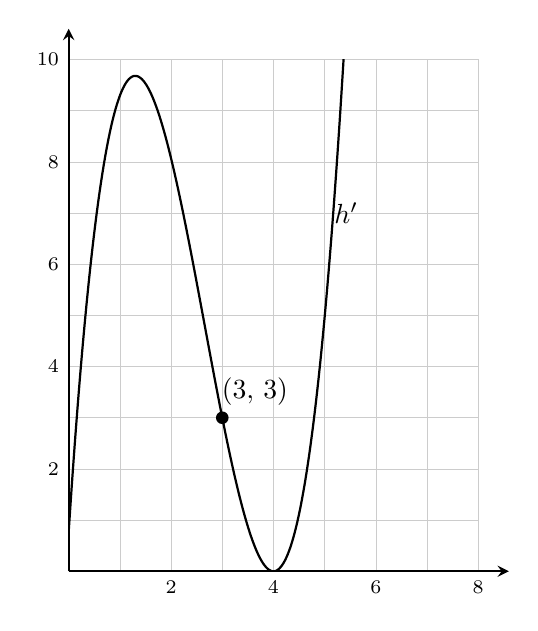
\begin{tikzpicture}[>=stealth, scale=0.65]
  % Grid
  \draw[step=1cm, gray!40, very thin] (0,0) grid (8,10);

  % Axes
  \draw[->, thick] (0,0) -- (8.6,0);
  \draw[->, thick] (0,0) -- (0,10.6);

  % x-axis tick labels (even values)
  \foreach \x in {2,4,6,8}
    \draw (\x,0) node[below, font=\scriptsize] {$\x$};
  % y-axis tick labels (even values)
  \foreach \y in {2,4,6,8,10}
    \draw (0,\y) node[left, font=\scriptsize] {$\y$};

  % Curve (clipped to the visible region)
  \begin{scope}
    \clip (0,0) rectangle (8,10);
    \draw[thick, ->] plot[domain=-0.25:5.42, samples=200, smooth]
      (\x, {2.95081967*((\x*\x*\x)/3 - 2.65*\x*\x + 5.2*\x) + 0.78688525});
  \end{scope}

  % Function label
  \node[anchor=west] at (5.0,7.0) {$h'$};

  % Filled dot at (3,3) with label
  \fill[black] (3,3) circle (3.5pt);
  \node[anchor=south west] at (2.80,3.05) {$(3,\,3)$};
\end{tikzpicture}
\end{document}
